%%%%%%%%%%%%%%%%%%%%%%%
%%% DOCUMENT SETTINGS
%%%%%%%%%%%%%%%%%%%%%%%
\documentclass[11pt]{exam}
\printanswers % Uncomment to show answers if desired
%%%%%%%%%%%%%%
%%% PACKAGES
%%%%%%%%%%%%%%
\usepackage{amsmath,amsfonts,amssymb,amsthm}  % math fonts and symbols
\usepackage{bbm} % Math blackboard font
\usepackage{enumitem} % Custom list environments
\usepackage{textcomp} % Misc symbols
\usepackage[top=2cm, bottom=2cm, right=1.2cm, left=1.2cm, paper=a4paper, headheight=6cm]{geometry} % Page layout
\usepackage{xcolor}  % Colors
\usepackage{graphicx} % Graphics
\usepackage{eurosym}
%----------------------------------- TikZ
\usepackage{tikz}
\usepackage{pgfplots}
\pgfplotsset{compat=1.17}
\usepgfplotslibrary{fillbetween}
\usetikzlibrary{shapes,arrows,matrix,positioning,calc}
\newcommand{\tikzmark}[1]{\tikz[baseline,remember picture] \coordinate (#1) {};}
%%%%%%%%%%%%%%%%%%%%%%%%%%
%%% COLORS
%%%%%%%%%%%%%%%%%%%%%%%%%%
\definecolor{brickred}{RGB}{200, 50, 50}
\definecolor{skyblue}{RGB}{0, 150, 220}
\definecolor{olivegreen}{RGB}{120, 160, 60}
%%%%%%%%%%%%%%%%%%%%%%%%%%
%%% MACROS
%%%%%%%%%%%%%%%%%%%%%%%%%%
\newcommand{\N}{\mathbb{N}} % natural numbers
\newcommand{\R}{\mathbb{R}} % real numbers
\makeatletter
\renewcommand{\@makefnmark}{\textsuperscript{\arabic{footnote}}}
\renewcommand{\thefootnote}{\arabic{footnote}}
\makeatother
\setcounter{footnote}{0}
\newcommand{\BAR}{%
  \hspace{-\arraycolsep}\strut\vrule\hspace{-\arraycolsep}}
%%%%%%%%%%%%%%%%%%%%%%%%%%%%%%%%%
%%% HEADER AND FOOTER
%%%%%%%%%%%%%%%%%%%%%%%%%%%%%%%%%
% Document information
\newcommand{\degree}{Bachelor in Philosophy, Politics and Economics}
\newcommand{\shortdeg}{PPE}
\newcommand{\exam}{Mock Exam 3}
\newcommand{\subject}{Mathematics}
\newcommand{\theyear}{2024/25}
\newcommand{\ccauthor}{A. G. Azze}
\newcommand{\thedate}{May 27, 2025}
\newcommand{\university}{CUENF Universidad}
% Set header and footer
\pagestyle{headandfoot}
\header{\degree \\ \subject\ - \theyear}{}{\thedate \\ \ccauthor}
\footer{\university}{}{\thepage}
%%%%%%%%%%%%%%%%%%%%%%%%%%
%%% DOCUMENT CONTENT
%%%%%%%%%%%%%%%%%%%%%%%%%%
\begin{document}
%--- Instructions ---%
\begin{center}
    {\Huge \textbf{\exam{}}}
    \begin{flushright}
        \vspace{-0.3cm}
        \textbf{Time Limit:} 120 minutes
    \end{flushright}
    \vspace{-0.1cm}
    \fbox{\parbox{\textwidth}{\centering 
        \begin{enumerate}[leftmargin=0.5cm, label=$\bullet$, rightmargin=0.2cm]
            \item Every non-trivial calculation and claim must be justified.
            % \item Calculators are not necessary and will not be allowed.
            \item Digital devices and internet access are prohibited.
        \end{enumerate}
    }}
\end{center}

%--- Questions ---%

\begin{questions}

%%%%%%%%%%%%%%%%%%%%%%%%%%%%%%%%%%%%%%%%%%%%%%%%%%%%%%%%%%%%%%%%%%%%%
% Question 1
%%%%%%%%%%%%%%%%%%%%%%%%%%%%%%%%%%%%%%%%%%%%%%%%%%%%%%%%%%%%%%%%%%%%%
\question[3]
In the market for premium organic coffee beans, the inverse demand and supply functions (in thousands) are:
\[
p_D(q)=22-q, \quad p_S(q)=2+q,
\]
where $q$ is quantity (in thousands of kg) and $p$ is price (in hundreds of euros) per kg.

\begin{minipage}{0.51\textwidth}
\begin{enumerate}[leftmargin=0.5cm, label=(\alph*), rightmargin=0.2cm]
    \item Find the market equilibrium $(q^*,p^*)$ without subsidy.
    \item Compute the producer surplus 
    $$
    PS = p^*q^*-\int_0^{q^*}p_S(q)\,dq.
    $$
    \item Highlight in Figure 1 the region whose are is given by $PS$. 
    \item Compute the area of region A in Figure 1.
    
\end{enumerate}
\end{minipage}
\hspace{0.8cm}
\begin{minipage}{0.35\textwidth}
\vspace{-0.1cm}
\begin{center}
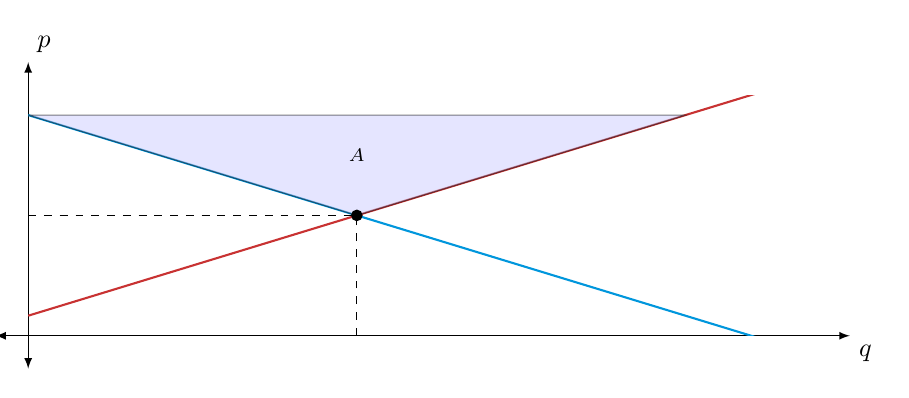
\begin{tikzpicture}[scale=0.95]
  \begin{axis}[
    width=\textwidth,
    height=4.8cm,
    axis lines=middle,
    xmin=0, xmax=24,
    ymin=0, ymax=24,
    xtick={0}, ytick={0},
    xlabel=$q$, ylabel=$p$,
    ticklabel style={font=\scriptsize},
    axis line style={latex-latex, shorten >=-12.5pt, shorten <=-12.5pt},
    xlabel style={at={(ticklabel* cs:1)}, xshift=12.5pt, anchor=north west},
    ylabel style={at={(ticklabel* cs:1)}, yshift=12.5pt, anchor=south west},
  ]
    % Demand and supply
    \addplot[thick, skyblue, samples=100, smooth, domain=0:24] {22 - x};
    \addplot[thick, brickred, samples=100, smooth, domain=0:24] {2 + x};
    % Equilibrium
    \addplot[mark=*, fill=black] coordinates {(10,12)};
    \addplot[dashed] coordinates {(10,0) (10,12)};  % vertical to q=10
    \addplot[dashed] coordinates {(0,12) (10,12)};  % horizontal to p=12
    % Region A: triangle between p-axis, demand curve, and q=10
    \addplot[fill=blue!20, opacity=0.5]
      coordinates { (0,22) (20,22) (10,12) } -- cycle;
    \node at (axis cs:10,18) {\scriptsize $A$};
  \end{axis}
\end{tikzpicture}
\vspace{-0.2cm}

{\small Figure 1}
\end{center}
\end{minipage}

A marketing campaign by producers increases consumers’ willingness to pay by $H$ (in hundreds of euros), so the new demand becomes
\[
p_D(q;H)=22 - q + H.
\]

\begin{enumerate}[label=(\alph*), leftmargin=0.5cm, start=5]
  \item What would be the new equilibrium ($q^*(H)$, $p^*(H)$)?
  \item What is the domain of the function $f(H) = 1/p^*(H)$?
  \item As a monopolist, what would be your net profit $P(H)$ after carrying out the marketing campaign, whose cost is $0.5H^2$, and profiting from selling out all the demanded quantity $q^*(H)$, each item at price $p^*(H)$?
  \item Find the value of $H$ that maximizes $P(H)$.
  \item Compute $P'(6)$ and use it to give a linear approximation for $M(6.1)$.
\end{enumerate}

\begin{solution}
\begin{enumerate}[label=(\alph*)]
  \item Solve $22-q=2+q$ gives $q^*=10$, $p^*=12$.
  \item $PS = 120-\int_0^{10}(2+q)\,dq=120-(20+50)=120-70=50.$
    \item The producer surplus region is the triangular area between the horizontal line \(p=12\) and the supply curve \(p_S(q)=2+q\) over \(0\le q\le10\).
  \item The shaded region $A$ is the triangle with vertices $(0,q_D(0) = 22)$, $(20,q_S(20) = 22)$, and $(q^*,p^*) = (10,12)$.
    Geometrically, its base is $20$ (from $q=0$ to $q=20$ at $p=22$) and its height is $10$ (from $p=12$ to $p=22$), so
    \[
    A \;=\; \frac12 \cdot 20 \cdot 10 \;=\; 100.
    \]

    Alternatively, $A$ can be written as the area between the horizontal line $p=22$ and the curves
    $p_D(q)=22-q$ on $[0,10]$ and $p_S(q)=2+q$ on $[10,20]$:
    \[
    A
    = \int_0^{10}\bigl[22 - (22 - q)\bigr]\,dq
      + \int_{10}^{20}\bigl[22 - (2 + q)\bigr]\,dq
    = \int_0^{10} q\,dq + \int_{10}^{20} (20 - q)\,dq
    = 50 + 50 = 100.
    \]

  \item New equilibrium solves 
    \[
      22 - q + H \;=\; 2 + q
      \;\Longrightarrow\;
      q^*(H)=10+\tfrac12H,
      \quad
      p^*(H)=12+\tfrac12H.
    \]
  \item $f(H)=\frac1{p^*(H)}$ is defined for $p^*(H)\neq0$, that is, $H\neq-24.$
  \item As a monopolist you earn revenue 
  \[
    R(H)=p^*(H)\,q^*(H)
           =(12+\tfrac H2)(10+\tfrac H2)
           =120 + 11H + \tfrac{H^2}4,
  \]
  and incur marketing cost \(\tfrac12H^2\).  Hence
  \[
    P(H)=R(H)-\tfrac12H^2
         =120 + 11H + \tfrac{H^2}4 \;-\;\tfrac{H^2}2
         =120 + 11H - \tfrac{H^2}4.
  \]
  \item Since $P'(H)=11 - \tfrac{H}{2}$, then $P'(H)=0\;\Longleftrightarrow H=22$. Since $P'(H) > 0$ for all $H < 22$ and $P'(H) < 0$ for all $H > 22$, then the profit is maximized at $H = 22$.
  \item $P'(6)=11 - \tfrac{6}{2}=11-3=8$. The linear approximation at \(H=6\) gives 
  $$
  P(6.1)\approx P(6) + P'(6)\,(0.1)
             =\bigl(-0.25\cdot6^2+11\cdot6+120\bigr)
              \;+\;8\cdot0.1
             =177 + 0.8
             =177.8.
  $$
\end{enumerate}
\end{solution}

%%%%%%%%%%%%%%%%%%%%%%%%%%%%%%%%%%%%%%%%%%%%%%%%%%%%%%%%%%%%%%%%%%%%%
% Question 2
%%%%%%%%%%%%%%%%%%%%%%%%%%%%%%%%%%%%%%%%%%%%%%%%%%%%%%%%%%%%%%%%%%%%%
\question[2]
A water‐treatment facility processes $3000$ L/day: $x$ to city, $y$ to irrigation, $z$ to cooling. Processing a L of water for the city earns $0.30$ euros, for irrigation costs $0.05$ euros, and for cooling earns 0.10 euros. The daily net‐revenue target is $800$ euros. On maintenance days, the processing capacity is reduced to two thirds for the city, one half for irrigation, and one fourth for cooling, and the target net revenue is $500$ euros.
\begin{enumerate}[label=(\alph*)]
  \item Write the system of linear equations in $x,y,z$.
  \item Express it in matrix form $Aw=b$ with $w=(x,y,z)^T$.
  \item Find the value of $x$, $y$ and $z$.
  \item If cooling and city processing capacities on maintenance days were reduced to one half instead, keeping the $500$ euros target, does a solution exist? Justify.
\end{enumerate}

\begin{solution}
\begin{enumerate}[label=(\alph*)]
  \item Regular: $0.3x-0.05y+0.1z=800$, $x+y+z=3000$.
    Maintenance: $0.3\tfrac23x-0.05\tfrac12y+0.1\tfrac14z=500$.
  \item $A=\begin{pmatrix}0.3&-0.05&0.1\\1&1&1\\0.2&-0.025&0.025\end{pmatrix},
    b=\begin{pmatrix}800\\3000\\500\end{pmatrix}.$
  \item Solve gives $(x,y,z)=(1500,1000,500)$.
  \item The new maintenance equation is $0.3\cdot\tfrac12x-0.05\cdot\tfrac12y+0.1\cdot\tfrac12z=500$, which is contradictory with the regular-day equation
\end{enumerate}
\end{solution}

%%%%%%%%%%%%%%%%%%%%%%%%%%%%%%%%%%%%%%%%%%%%%%%%%%%%%%%%%%%%%%%%%%%%%
% Question 3
%%%%%%%%%%%%%%%%%%%%%%%%%%%%%%%%%%%%%%%%%%%%%%%%%%%%%%%%%%%%%%%%%%%%%
\question[3]
A swimmer in distress is located offshore at point $S$. The closest point $C$ to the swimmer on the shoreline is 9 meters away, measured perpendicular to the shore. A lifeguard is on the shore at point \(L\), 8 meters away from $C$. The shore is a straight line.

The lifeguard can run along the beach at 16 m/s (up to 8m) and swim at 4 m/s. She decides to run \(x\) m downshore from \(L\), then swim straight toward the swimmer, so that the total time to reach the swimmer is, in seconds,
\[
T(x) \;=\; \frac{x}{16} \;+\; \frac{\sqrt{(8 - x)^2 + 81}}{4}.
\]

\begin{enumerate}[label=(\alph*)]
  \item How long it would take if she decides to enter the water immediately? and if she runs for $8$km before jumping into the water?
  \item How many meters \(x\) should she run to minimize the time to the swimmer? What is the minimal time?
  \item If entry to the water is forbidden before $6$ meters, what $x$ minimizes $T(x)$ now?
\end{enumerate}

\begin{solution}
\begin{enumerate}[label=(\alph*)]
  \item $T(0)=\tfrac{9}{4}=2.25$ h, 
    $T(8)=\tfrac{8}{16}+\tfrac{9}{4}=0.5+2.25=2.75$ seconds.
  \item Since $T'(x)=\frac1{16}-\frac{8-x}{4\sqrt{(8-x)^2+81}}$, then  
  \begin{align*}
        T'(x)=0 &\Longleftrightarrow 
        \frac1{16}=\frac{8-x}{4\sqrt{(8-x)^2+81}}
        \;\Longleftrightarrow\;
        16(8-x)=4\sqrt{(8-x)^2+81}. \\
        &\Longleftrightarrow
        15(8-x)^2=81
        \;\Longrightarrow\;
        (8-x)^2=\frac{27}{5},
        \qquad
        8-x=\sqrt{\tfrac{27}{5}}.
  \end{align*}
    Hence $x^* = 8-\sqrt{\tfrac{27}{5}}$. Since $T'(x) < 0$ for all $x \in [0, x^*)$ and $T'(x) > 0$ for all $x \in (x^*, 8)$, then $x^*$ is the global minimizer. Evaluating the minimal time:
    $$
    T_{\min}=T(x^*)=\frac{8-\sqrt{27/5}}{16}
              +\frac{\sqrt{(27/5)+81}}{4}
            =\frac{8-\sqrt{27/5}}{16}
              +3\sqrt{\tfrac{3}{5}}
            \approx \boxed{\,2.679\text{ s}\,}.
    $$
  \item For $x\ge6$, the best running distance is at boundary $x=6$, since $T(x)$ is decreasing in the interval $[6, 8]$.
\end{enumerate}
\end{solution}

%%%%%%%%%%%%%%%%%%%%%%%%%%%%%%%%%%%%%%%%%%%%%%%%%%%%%%%%%%%%%%%%%%%%%
% Question 4
%%%%%%%%%%%%%%%%%%%%%%%%%%%%%%%%%%%%%%%%%%%%%%%%%%%%%%%%%%%%%%%%%%%%%
\question[2]
A hydroelectric dam’s daily output $E(t)$ (for $t$ representing days, and output given in kWh) increases over time due to continuous improvements of the facility, so that
\[
E(t) = 50(1+ 0.1t)
\quad(\text{kWh in month }t).
\]
If the market price per kWh in month \(t\) is \(M(t)\) dollars, total revenue over \(T\) days is
\[
R(T) \;=\; \int_{0}^{T} E(t)\,M(t)\,\mathrm{d}t.
\]
\begin{enumerate}[label=(\alph*)]
  \item If \(M(t)=1\), compute the revenue after \(120\) days.
  \item Compute the perpetual revenue \(\displaystyle\lim_{T\to\infty}R(T)\) if \(M(t)\) if $M(t) = (1+ 0.1t)^{-2}$. Hint: what is the derivative of $\ln(1 + 0.1t)$?
  \item If \(M(t)=1\), how long until the revenue reaches \(750\)?
\end{enumerate}

\begin{solution}
\begin{enumerate}[label=(\alph*)]
\item 
\[
\begin{aligned}
R(120)&=\int_{0}^{120} 50\bigl(1+0.1t\bigr)\,dt
      =50\Bigl[t+0.05t^{2}\Bigr]_{0}^{120}   \\
      &=50\bigl(120+0.05\cdot 120^{2}\bigr)
      =50(120+720)=\boxed{42\,000}.
\end{aligned}
\]
Thus the revenue after \(120\) days is \$42\,000.

%-------------------------------------------------
\item 
\begin{align*}
    R(T) &=\int_{0}^{T} 50\,(1+0.1t)\,(1+0.1t)^{-2}\,dt
          =50\int_{0}^{T}\frac{dt}{1+0.1t} \\
        &= 500\ln\!\bigl(1+0.1T\bigr)
\end{align*}
Hence
\[
\lim_{T\to\infty}R(T)=\lim_{T\to\infty}500\ln\!\bigl(1+0.1T\bigr)=\infty,
\]
so the perpetual revenue diverges.

%-------------------------------------------------
\item $R(T)=50T+2.5T^{2}$. Hence,
\begin{align*}
    R(T)=750 &\Longleftrightarrow 2.5T^{2}+50T-750=0
    \Longleftrightarrow T^{2}+20T-300=0. \\
    &\Longleftrightarrow (T+30)(T-10) = 0
\end{align*}
Hence, since $T$ must be positive, the solution is $T = 10$. That is, the hydroelectric will reach $750$ dollars of revenue after 10 days.
\end{enumerate}
\end{solution}

\end{questions}
\end{document}
